% Sketch output, version 0.3 (build 2d, Wed Apr 20 23:38:45 2011)
% Output language: PGF/TikZ,LaTeX
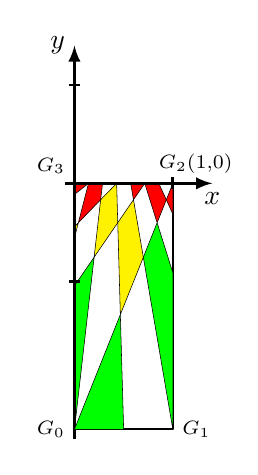
\begin{tikzpicture}[line join=round,line width=0.2pt,>=latex]
\filldraw[fill=none,line width=0.75pt](7,-7.125)--(8.25,-7.125)--(8.25,-4)--(7,-4)--cycle;
\filldraw[fill=yellow](7.333,-4.208)--(7.25,-4.938)--(7.55,-4.5)--(7.536,-4)--cycle;
\filldraw[fill=red](7,-4)--(7,-4.142)--(7.179,-4)--cycle;
\filldraw[fill=red](7.179,-4)--(7.05,-4.5)--(7.333,-4.208)--(7.357,-4)--cycle;
\filldraw[fill=red](8.25,-4.391)--(8.25,-4)--(8.167,-4.208)--cycle;
\filldraw[fill=red](8.05,-4.5)--(8.167,-4.208)--(8.071,-4)--(7.893,-4)--cycle;
\filldraw[fill=red](7.714,-4)--(7.75,-4.208)--(7.893,-4)--cycle;
\filldraw[fill=yellow](7.583,-5.667)--(7.875,-4.938)--(7.75,-4.208)--(7.55,-4.5)--cycle;
\filldraw[fill=yellow](7.05,-4.5)--(7,-4.694)--(7,-4.551)--cycle;
\filldraw[fill=green](8.25,-7.125)--(8.25,-5.136)--(8.05,-4.5)--(7.875,-4.938)--cycle;
\filldraw[fill=green](7,-7.125)--(7.25,-4.938)--(7,-5.302)--cycle;
\draw[->,line width=1pt](6.875,-4)--(8.75,-4);
\draw[->,line width=1pt](7,-7.25)--(7,-2.25);
\draw[line width=1pt](8.25,-3.925)--(8.25,-4.075);
\draw[line width=1pt](7.075,-2.75)--(6.925,-2.75);
\draw[line width=1pt](7.075,-5.25)--(6.925,-5.25);
\filldraw[fill=green](7,-7.125)--(7.625,-7.125)--(7.583,-5.667)--cycle;

    \coordinate [label=below:$x$] (X) at (8.75,-4);
    \coordinate [label=left:$y$] (Y) at (7,-2.25);
  
    \coordinate [label=180:\scriptsize$G_0$] (p0G) at (7,-7.125);
    \coordinate [label=  0:\scriptsize$G_1$] (p1G) at (8.25,-7.125);
    \coordinate [label= 90:{\scriptsize$G_2\makebox[0pt][l]{(1,0)}$}] (p2G) at (8.25,-4);
    \coordinate [label=135:\scriptsize$G_3$] (p3G) at (7,-4);
  \end{tikzpicture}% End sketch output
